\section{Search for MobileNetV3}

\subsection*{Abstract}

We present the next generation of MobileNets based on a combination of complementary search techniques as well
as a novel architecture design. MobileNetV3 is tuned to mobile phone CPUs through a combination of hardwareaware
network architecture search (NAS) complemented by the NetAdapt algorithm and then subsequently improved
through novel architecture advances. This paper starts the exploration of how automated search algorithms and network
design can work together to harness complementary approaches improving the overall state of the art. Through
this process we create two new MobileNet models for release: MobileNetV3-Large and MobileNetV3-Small which
are targeted for high and low resource use cases. These models are then adapted and applied to the tasks of object
detection and semantic segmentation. For the task of semantic segmentation (or any dense pixel prediction), we
propose a new efficient segmentation decoder Lite Reduced Atrous Spatial Pyramid Pooling (LR-ASPP). We achieve
new state of the art results for mobile classification, detection and segmentation. MobileNetV3-Large is 3.2% more
accurate on ImageNet classification while reducing latency by 20\% compared to MobileNetV2. MobileNetV3-Small is
6.6\% more accurate compared to a MobileNetV2 model with comparable latency. MobileNetV3-Large detection
is over 25\% faster at roughly the same accuracy as MobileNetV2 on COCO detection. MobileNetV3-Large LRASPP
is 34\% faster than MobileNetV2 R-ASPP at similar accuracy for Cityscapes segmentation.

\begin{figure}[!htbp]
    \centering
    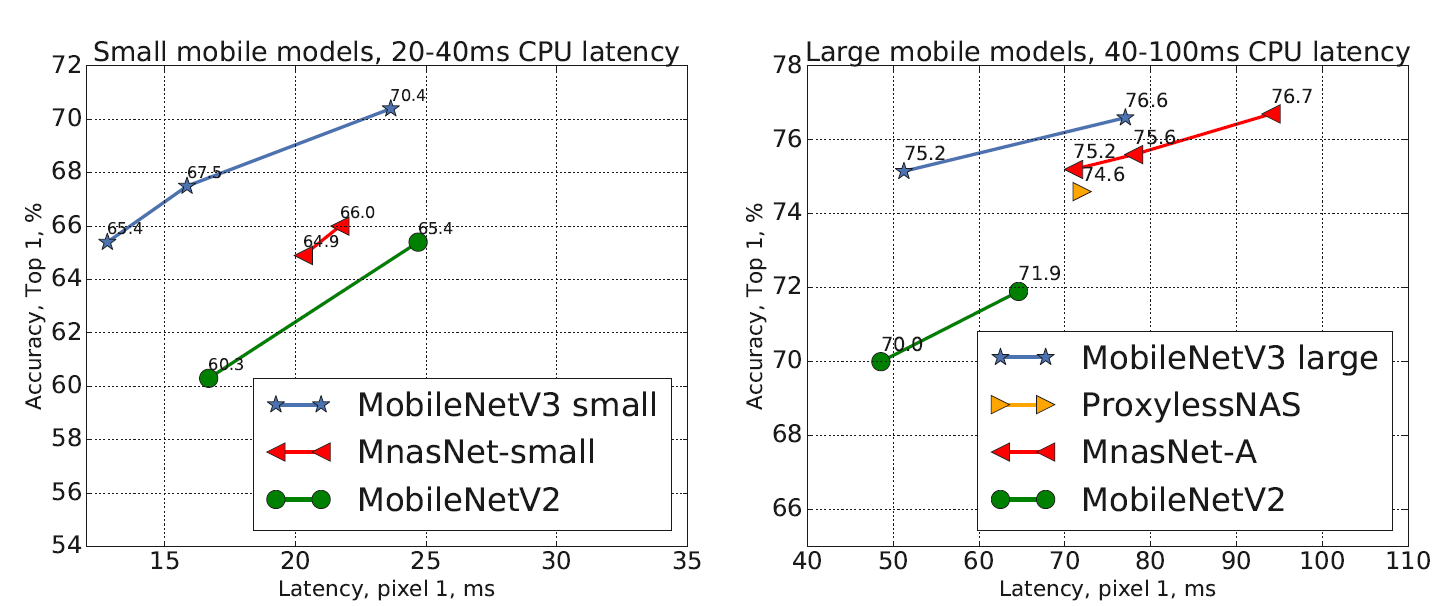
\includegraphics[width=5in]{Figure1.png}
    \caption{The trade-off between Pixel 1 latency and top-1 ImageNet accuracy. All models use the input resolution 224. V3 large
    and V3 small use multipliers 0.75, 1 and 1.25 to show optimal frontier. All latencies were measured on a single large core of the
    same device using TFLite[1]. MobileNetV3-Small and Large are our proposed next-generation mobile models.}
\end{figure}

\begin{figure}[!htbp]
    \centering
    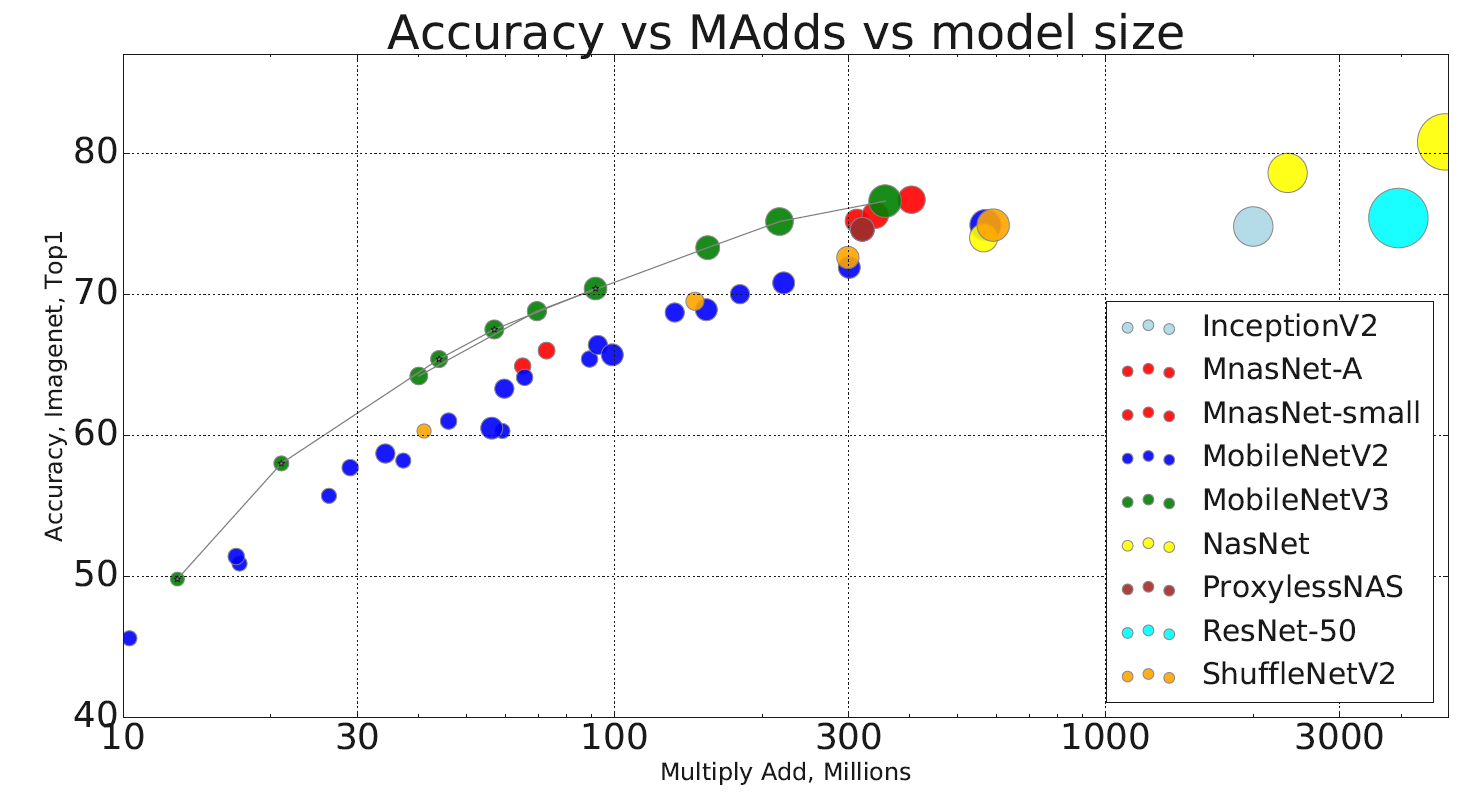
\includegraphics[width=5in]{Figure2.png}
    \caption{The trade-off between MAdds and top-1 accuracy. This allows to compare models that were targeted different hardware or
    software frameworks. All MobileNetV3 are for input resolution 224 and use multipliers 0.35, 0.5, 0.75, 1 and 1.25. See section 6
    for other resolutions. Best viewed in color.}
\end{figure}


\subsection{Intrudction}

Efficient neural networks are becoming ubiquitous in mobile applications enabling entirely new on-device experiences.
They are also a key enabler of personal privacy allowing a user to gain the benefits of neural networks without
needing to send their data to the server to be evaluated. Advances in neural network efficiency not only improve user
experience via higher accuracy and lower latency, but also help preserve battery life through reduced power consumption.

This paper describes the approach we took to develop MobileNetV3 Large and Small models in order to deliver
the next generation of high accuracy efficient neural network models to power on-device computer vision. The new
networks push the state of the art forward and demonstrate how to blend automated search with novel architecture advances
to build effective models.

The goal of this paper is to develop the best possible mobile computer vision architectures optimizing the accuracylatency
trade off on mobile devices. To accomplish this we introduce (1) complementary search techniques, (2) new efficient
versions of nonlinearities practical for the mobile setting, (3) new efficient network design, (4) a new efficient
segmentation decoder. We present thorough experiments demonstrating the efficacy and value of each technique evaluated
on a wide range of use cases and mobile phones.

The paper is organized as follows. We start with a discussion of related work in Section 2. Section 3 reviews the
efficient building blocks used for mobile models. Section 4 reviews architecture search and the complementary nature
of MnasNet and NetAdapt algorithms. Section 5 describes novel architecture design improving on the efficiency of the
models found through the joint search. Section 6 presents extensive experiments for classification, detection and segmentation
in order do demonstrate efficacy and understand the contributions of different elements. Section 7 contains
conclusions and future work.

\subsection{Relate Work}

Designing deep neural network architecture for the optimal trade-off between accuracy and efficiency has been
an active research area in recent years. Both novel handcrafted structures and algorithmic neural architecture search
have played important roles in advancing this field.

SqueezeNet[22] extensively uses 1x1 convolutions with squeeze and expand modules primarily focusing on reducing
the number of parameters. More recent works shifts the focus from reducing parameters to reducing
the number of operations (MAdds) and the actual measured latency. MobileNetV1[19] employs depthwise separable
convolution to substantially improve computation efficiency. MobileNetV2[39] expands on this by introducing
a resource-efficient block with inverted residuals and linear bottlenecks. ShuffleNet[49] utilizes group convolution
and channel shuffle operations to further reduce the MAdds. CondenseNet[21] learns group convolutions at the training
stage to keep useful dense connections between layers for feature re-use. ShiftNet[46] proposes the shift operation interleaved
with point-wise convolutions to replace expensive spatial convolutions.

To automate the architecture design process, reinforcement learning (RL) was first introduced to search efficient
architectures with competitive accuracy [53, 54, 3, 27, 35]. A fully configurable search space can grow exponentially
large and intractable. So early works of architecture search focus on the cell level structure search, and the same cell is
reused in all layers. Recently, [43] explored a block-level hierarchical search space allowing different layer structures
at different resolution blocks of a network. To reduce the computational cost of search, differentiable architecture
search framework is used in [28, 5, 45] with gradient-based optimization. Focusing on adapting existing networks to
constrained mobile platforms, [48, 15, 12] proposed more efficient automated network simplification algorithms.

Quantization [23, 25, 47, 41, 51, 52, 37] is another important complementary effort to improve the network
efficiency through reduced precision arithmetic. Finally, knowledge distillation [4, 17] offers an additional complementary
method to generate small accurate ”student” networks with the guidance of a large ”teacher” network.

\subsection{Efficient Mobile Building Blocks}

Mobile models have been built on increasingly more efficient building blocks. MobileNetV1 [19] introduced depthwise
separable convolutions as an efficient replacement for traditional convolution layers. Depthwise separable convolutions
effectively factorize traditional convolution by separating spatial filtering from the feature generation mechanism.
Depthwise separable convolutions are defined by two separate layers: light weight depthwise convolution for
spatial filtering and heavier 1x1 pointwise convolutions for feature generation.

MobileNetV2 [39] introduced the linear bottleneck and inverted residual structure in order to make even more efficient
layer structures by leveraging the low rank nature of the problem. This structure is shown on Figure 3 and is
defined by a 1x1 expansion convolution followed by depthwise convolutions and a 1x1 projection layer. The input and
output are connected with a residual connection if and only if they have the same number of channels. This structure
maintains a compact representation at the input and the output while expanding to a higher-dimensional feature space
internally to increase the expressiveness of nonlinear perchannel transformations.

MnasNet [43] built upon the MobileNetV2 structure by introducing lightweight attention modules based on squeeze
and excitation into the bottleneck structure. Note that the squeeze and excitation module are integrated in a different
location than ResNet based modules proposed in [20]. The module is placed after the depthwise filters in the expansion
in order for attention to be applied on the largest representation as shown on Figure 4.

For MobileNetV3, we use a combination of these layers as building blocks in order to build the most effective models.
Layers are also upgraded with modified swish nonlinearities [36, 13, 16]. Both squeeze and excitation as well as
the swish nonlinearity use the sigmoid which can be inefficient to compute as well challenging to maintain accuracy
in fixed point arithmetic so we replace this with the hard sigmoid [2, 11] as discussed in section 5.2.

\begin{figure}[!htbp]
    \centering
    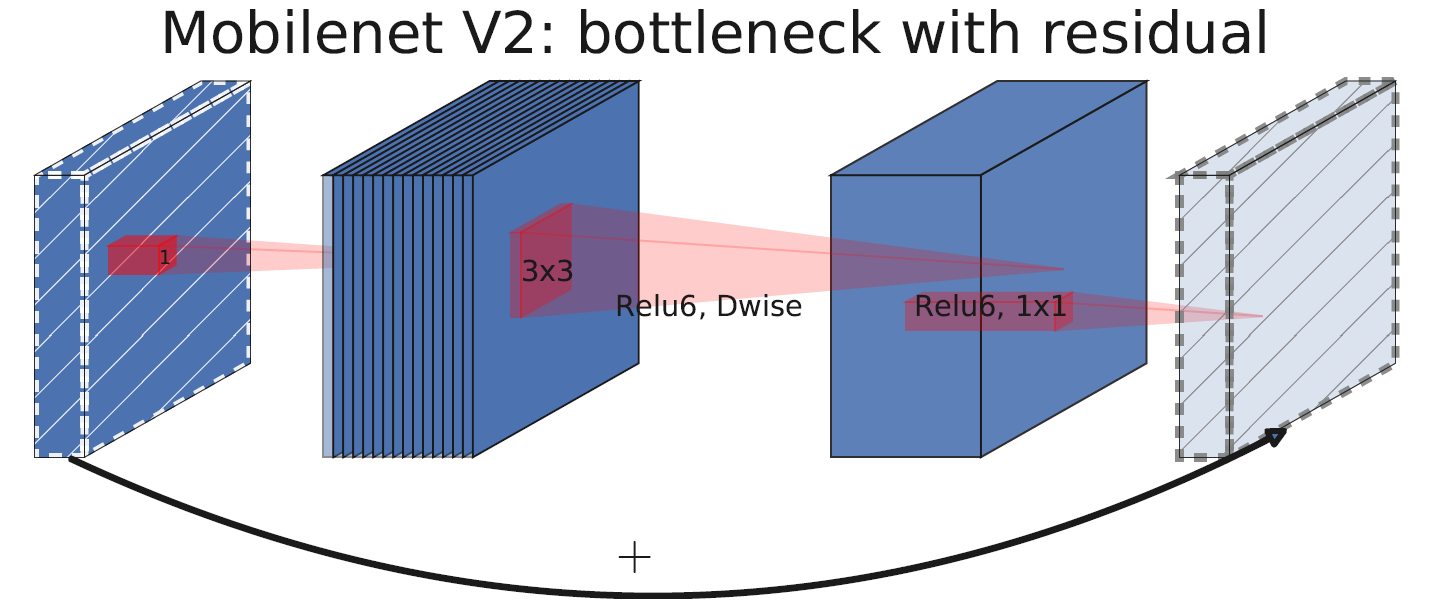
\includegraphics[width=5in]{Figure3.png}
    \caption{MobileNetV2 [39] layer (Inverted Residual and LinearBottleneck). Each block consists of narrow input and output (bottleneck),
    which don’t have nonlinearity, followed by expansion to a much higher-dimensional space and projection to the output. The
    residual connects bottleneck (rather than expansion).}
\end{figure}


\begin{figure}[!htbp]
    \centering
    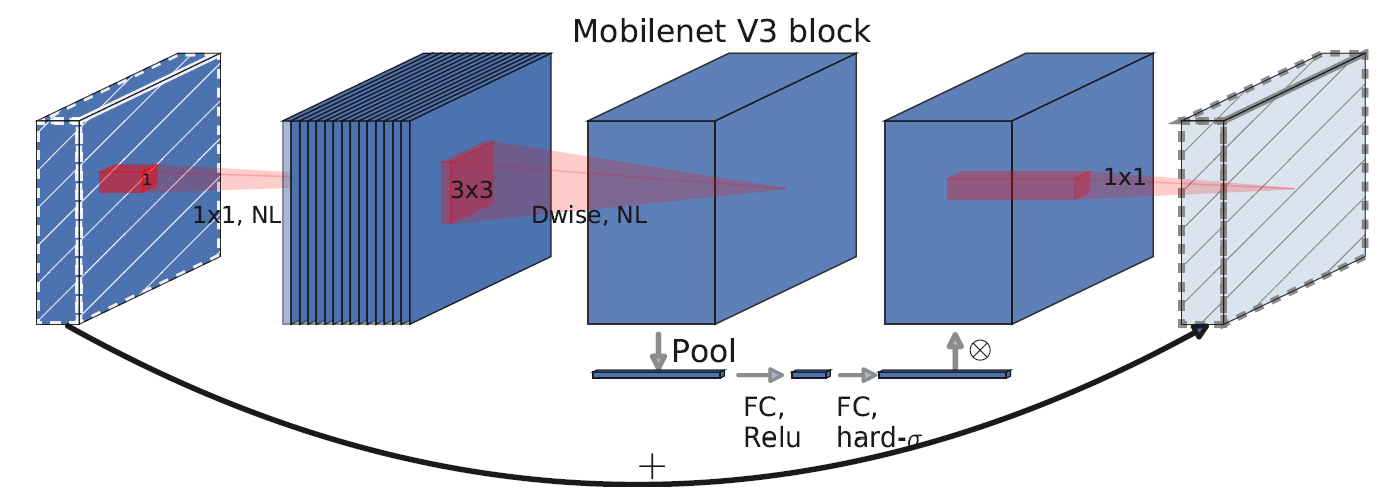
\includegraphics[width=5in]{Figure4.png}
    \caption{MobileNetV2 + Squeeze-and-Excite [20]. In contrast with [20] we apply the squeeze and excite in the residual layer.
    We use different nonlinearity depending on the layer, see section 5.2 for details.}
\end{figure}